\documentclass[fleqn,10pt]{wlpeerj}
\title{Comprehensive, structurally-curated alignment and phylogeny of Vertebrate biogenic amine receptors}

\author[1,2,3]{Stephanie J. Spielman}
\author[4,5]{Ahmad R. Sedaghat}
\author[1,2,3]{Keerthana Kumar}
\author[1,2,3]{Claus O. Wilke}
\affil[1]{Department of Integrative Biology, The University of Texas at Austin, Austin, U.S.A.}
\affil[2]{Institute of Cellular and Molecular Biology, The University of Texas at Austin, Austin, U.S.A.}
\affil[3]{Center for Computational Biology and Bioinformatics, The University of Texas at Austin, Austin, U.S.A.}
\affil[4]{Department of Otolaryngology–Head and Neck Surgery, Massachusetts Eye and Ear Infirmary, Boston, Massachusetts, U.S.A.}
\affil[5]{Department of Otology and Laryngology, Harvard Medical School, Boston, Massachusetts, U.S.A.}

\keywords{biogenic amine receptors, phylogenetics, multiple sequence alignment, G-protein coupled receptors}


\begin{abstract}


\end{abstract}

\begin{document}

\flushbottom
\maketitle
\thispagestyle{empty}


\section*{Introduction}

Biogenic amines, such as the molecules serotonin and dopamine, play critical roles in virtually all Metazoa taxa, exerting significant influence on both behavior and physiology. In vertebrates, these molecules' actions are mediated primarily through the biogenic amine receptor family, which includes dopamine (DRD), histamine (HRH), trace (TAAR), adrenergic (ADR), muscarinic cholinergic (mAChR), and most serotonin receptors (5HTR).  Biogenic amine receptors belong to the broad family of G protein-coupled receptors (GPCRs), one of the largest and most diverse receptor families in eukaryota, and indeed Metazoa. Indeed, due to the extensive diversity of biological functions they direct and the ongoing expansion of their ligand repertoire, GPCRs are considered one of the most evolutionarily innovative and successful gene families \citep{BockaertPin1999,Lagerstrom2008}.

Biogenic amine receptors form a clade within large the Rhodopsin-like (family ``A'') GPCR family, whose emergence likely accompanied that of the Opisthokont (Fungi and Metazoa) lineage \citep{Krishnan2012}. Subsequently, the Rhodopsin-like family underwent substantial expansion in Metazoa, most notably in Vertebrate lineages \citep{Rompleretal2007,Staubert2013}. Like all GPCRs, these receptors contain a highly-conserved, characteristic GPCR structure of seven transmembrane (TM) domains separated by three extracellular (ECL) and three intracellular (ICL) loops, and they propagate intracellular signaling through a G protein-mediated pathway. Biogenic amine receptors are prominent targets for a wide array of pharmaceuticals aimed to treat myriad diseases such as schizophrenia, migraines, hypertension, allergies and asthma, and stomach ulcers \citep{Schoneberg2004,Eversetal2005,Masonetal2012}.

In spite of these receptors' biological and clinical importance, studies on their evolution are relatively limited. Evolutionary studies which have focused on a biogenic amine receptors have predominantly been limited to single receptor subtypes, namely TAAR \citep{Gloriametal2005,Lindemann2005,Hashiguchi2007}, DRD \citep{Callieretal2003,Yamamotoetal2013}, and 5HTR \cite{Anbazhagan2010}. Moreover, many of these studies, and indeed larger-scale studies on the general evolution of the Rhodopsin-like GPCR family, have examined very narrow species distributions, for instance specifically teleosts \citep{Gloriametal2005}, primates \citep{Anbazhagan2010}, humans and mice \citep{Vassilatis2003,KakaralaJamil2014}, or even strictly humans \cite{Fredrikssonetal2003}. Thus, studies which account for the full breadth of known bioamine receptor sequences as well as their broad species distributions remain elusive.

This dearth of biogenic amine receptor-specific evolutionary understanding is underscored by the difficulties in establishing a robust multiple sequence alignment (MSA). MSAs provide the founation for nearly all comparative sequence analyses, and they are commonly used to locate conserved sequence motifs, identify functionally important residues, and investigate the evolutionary histories. As constructing an MSA represents the first step in any sequence analysis, MSA errors are known to bias these downstream analyses \citep{Ogden2006, Wong2008, Jordan2012}. It is therefore crucial to ensure accuracy in MSAs to the extent possible. For GPCR sequences, in particular, any MSA should recapitulate the canonical 7TM structure, which a naive alignment of sequences cannot necessarily accomplish. While there are certain MSA software platforms that explicitly incorporate structural information into the alignment algorithm (e.g.\ 3DCoffee \citep{3dcoffee} and PROMALS3D \citep{promals3d}), these programs are fairly computationally-intensive and thus ill-suited for large-scale (over 1000 sequences) applications. Moreover, such programs require the use of a single crystal structure to guide sequence alignment. While all GPCRs have the same conserved 7TM domains, different GPCR subfamilies, particularly the biogenic amine receptors, feature a wide variety of ICL and ECL sizes. For instance, the ECL3 lengths for human HRH1 and DRD3, respectively, are roughly 27 and 117, and their respective ICL3 lengths are 68 and 14 (as predicted by GPCRHMM \citep{Wistrand2006}). Thus, aligning with a single crystral structure will not effectively represent the domain variability across biogenic amine receptor subtypes. A desirable alignment strategy would instead anchor all sequences by their conserved 7TM domains without inappropriately constraining the heterogeneous ECL and ICL domains.

We therefore have adopted a novel iterative alignment strategy to create a large (3064 sequences), structurally-curated MSA of vertebrate biogenic amine receptors. In order to ensure proper structural alignment, we employed the software GPCRHMM \citep{Wistrand2006}, which uses a hidden markov model approach to assign each residue in a given GPCR sequence to its respective domain, either extracellular, transmembrane, or intracellular. Previously validated with resolved Rhodopsin-like GPCR crystal structures \citep{SpielmanWilke2013}, GPCRHMM relies on the remarkably-conserved GPCR 7TM structure to predict GPCR domains from protein sequence alone with exceptional accuracy. Our alignment strategy therefore ensured that all predicted 7TM domains aligned appropriately across all sequences. Importantly, this strategy did not require any manual or visual data inspection, thus avoiding any confounding subjectivity in MSA processing. Moreover, to demonstrate the utility of our alignment, we constructed a phylogeny of our receptors with this alignment as well as a naive MSA which did not undergo this iterative process. We found that our structurally-curated MSA offered dramatic improvements in phylogenetic fit relative to a structurally-naive MSA. Furthermore, through this structurally-aware phylogeny, we are able to discern relationships among biogenic amine receptor subtypes with a far increased level of sensitivitiy relative to previous studies. We additionally identify novel lineage-specific receptor clades and clarify NCBI annotations for over 30 sequences. 

We present this large, taxonomically-comprehensive vertebrate biogenic receptor MSA and its corresponding phylogeny as a resource for any group interested in studying the dynamic evolutionary processes, structural, and/or functional constraints operating within this exceptionally important GPCR clade. All data, including MSAs, phylogenies, and sequence descriptions, as well as all code used to generate these data freely available from \texttt{https://github.com/sjspielman/amine\_receptors}. This structurally-aware MSA and corresponding phylogeny represent the most comprehensive and curated vertebrate biogenic amine receptor dataset to date and should therefore be extremely useful for studying both the broad patterns governing this biogenic amine receptor sequence evolution as well as receptor-specific evolutionary trends. Further, our curated MSA should may serve as a helpful resource in the ongoing development of homology models and pharmaceutical therapeutics targeting these receptors \citep{Kristiansen2004,Ishiguro2004,Eversetal2005,Masonetal2012}.




\section*{Results}

\subsection*{Constructing a structurally-curated MSA of biogenic amine receptors}
We collected all sequences using PSI-BLAST and filtered data to exclude poor-quality sequences and/or sequences with excessive ambiguities to ensure a high-quality data set (see \emph{Methods} for details). We additionally retained only sequences that could be unequivocally classified as GPCRs using the program GPCRHMM \citep{Wistrand2006}, leaving a total dataset of 3464 receptor sequences to align. We then built a structurally-curated MSA from these 3464 receptor protein sequences according to the iterative strategy outlined in Figure~\ref{flowchart}. Before aligning sequences, we again used the program GPCRHMM \citep{Wistrand2006} to assign each residue in all protein sequences to its respective structural domain (extracellular, transmembrane, or intracellular) using a $0.5$ posterior probability cutoff. Next, for each iteration of the algorithm in Figure~\ref{flowchart}, we aligned protein sequences with MAFFT \citep{mafftv7}. Using the GPCRHMM-derermined residue domains, we assigned a consensus structural domain to each MSA column. We then discarded all sequences for which $\geq 5\%$ of residues did not correspond to their respective column's consensus domain. We realigned the remaining sequences with MAFFT and continued in this manner until no more sequences were discarded, resulting in a structurally-curated MSA of 3039 sequences.

Using this final MSA, we additionally created a ``masked'' MSA in which protein residues which did not conform to their respective consensus domains were replaced with a ``?''. By replacing these positions with an ambiguous character, we ensuring that each MSA column strictly contained residues belonging to the same structural domain. In total, 2.69\% of all MSA positions were were masked in this second structural MSA. These final structurally-curated masked and unmasked MSAs contained a total of 3039 sequences. Figure~\ref{taxa_dist} displays the overall taxonomic distribution of sequences in these MSAs. 


\subsection*{Structurally-aware approach strongly improves phylogenetic inference}

To demonstrate the utility of analyzing biogenic amine receptors data with a structurally-curated MSA, we constructed five distinct maximum likelihood (ML) phylogenies, as detailed in Table~\ref{tab:phylo_AIC}, in RAxML. First, we built a phylogeny using an MSA, again built with MAFFT \citep{mafftv7}, comprised of the full set of 3464 receptors; in other words, this MSA was not subjected to the iterative process shown in Figure~\ref{flowchart}. As this MSA was not structurally-curated, we refer to it as the ``naive'' MSA. We additionally constructed two phylogenies each from the structural unmasked and masked MSAs. Previous work has shown that both structural and functional constraints impose differing selection pressures in TM vs.\ extramembrane (EM), which consists of both extracellular and intracellular, domains, additionally producing distinct amino-acid frequency distributions in each domain class \cite{Tourasse2000,Stevens2001,Julenius2006,Oberai2009,SpielmanWilke2013,FranzosaXueXia2013}. As our structurally-curated MSAs allow us to precisely identify each MSA column as either TM or EM, we can conduct far more rigorous phylogentic inference using a partition analysis. Therefore, for each of our two structurally-curated MSAs (masked and unmasked), we inferred two ML phylogenies: one with two partitions representing TM and EM columns and one with a single partition for the entire alignment. Importantly, such a partitioned analysis would not be possible without a structurally-curated MSA, as we present here.

As assessed by AIC scores, the structurally-curated masked MSA yielded a far superior phylogeny compared to all other MSAs (Table~\ref{tab:phylo_AIC}), highlighting the benefits of structurally-aware analyses. That the masked structural MSA produced phylogenies with substantially better fits than did the unmasked MSA underscores that any structurally-aware study must be undertaken cautiously. While partitioning the MSA based on structural domains was clearly benefically, ensuring that each MSA column contained strictly residues belonging to the same domain was critical. Having even a few TM residues in a column assigned to the EM partition, or vice versa, strongly hindered phylogenetic fit, explaining the improved performance of the masked structural MSA.



\subsection*{Structurally-aware phylogeny reveals unknown biogenic amine receptor relationships and clades}

Our resulting phylogeny, shown in Figure~\ref{phylogeny}, represents the most comprehensive and curated vertebrate biogenic amine receptor phylogeny to date. This tree broadly captures many known features of biogenic amine receptor evolution, in particular that these receptors do not cluster based on ligand-binding but rather have undergone extensive functional convergent evolution. Indeed, our phylogeny reveals that only two ligand-based receptor classes, mAChR and TAAR, are truly monophyletic. Using this phylogeny, we were able to reclassify several misannotated sequences (Table S1) as well as uncover an entirely unknown clade of biogenic amine receptors. This unknown clade, sister to HRH2, contains strictly avian sequences as well as one \emph{Xenopus tropicalis} sequence. Two evolutionary scenarios may explain this taxonomic distribution: either this clade emerged after the divergence of teleosts but was secondarily lost in Reptilia and Mammalia, or this clade represents an avian-specific diversification which the \emph{Xenopus tropicalis} sequence resembles only convergently. Interestingly, the vast majority of sequences in this clade were annotated in NCBI as either octopamine or No9-like receptors, both of which are insect-specific biogenic amine receptors that do not occur in vertebrate taxa. This sequence misannotation reveals an intriguing case of convergent evolution and suggests the hypothesis that these receptors may interact with atypical ligands in vertebrate lineages.

Our phylogeny features remarkably high bootstrap support for each distinct clade of receptor subtypes. We additionally find very strong support for three deeper nodes in the phylogeny that reveal the relationships among distinct receptor subtypes. The first contains the three clades HRH1, mAChR, and HRH-3,4, the second contains the clades 5HTR-1, 5HTR-5, and 5HTR-7, and finally the third contains the 5HTR-4 and TAAR clades. Previous studies have yielded conflicting phylogenetic placements for the 5HTR-7 clade; some have argued that 5HTR-7 is phylogenetically distinct from all other 5HTR sequences \citep{KakaralaJamil2014}, while others have found that evidence for a single clade containing 5HTR-5,7 as a sister taxa to a clade containing ADRA1 sequences \citep{Fredrikssonetal2003}. Alternatively, we find moderate-to-strong support for the 5HTR-7 clade having originated before subsequent diversification into 5HTR-5 and 5HTR-1, and we find full support showing that ADRA1 sequences form an entire distinct monophyletic group outside all other vertebrate biogenic amine receptors. In addition, as previously mentioned, our phylogeny reveals that HRH-3,4 is actually single monophyletic group. Moreover, the HRH-4 clade contains strictly mammalians sequences, including monotreme sequences, wheres the HRH-3 sequences are broadly distributed among vertebrate taxa. We therefore hypothesize that HRH-4 arose from an HRH-3 duplication concurrent with mammalian origins.

Of particular interest in our phylogeny are the unique evolutionary patterns revealed within the TAAR clade. While TAAR sequences do cluster together, the relationships among TAAR subtypes are highly dynamic, reflecting the extensive expansion and contraction events characterizing this receptor family's evolution \citep{Lindemann2005,Hashiguchi2007,Staubert2010,Staubert2013}. Figure~\ref{taar_tree} displays the subtree containing specifically TAAR sequences and in fact differs somewhat from previously proposed TAAR trees \citep{Lindemann2005, Hashiguchi2007}. In particular, the presence of several lineage-specific subclades as well as unresolved subclades generate novel hypotheses regarding TAAR subtype origins. While TAAR-2,3,4 form a well-resolved monophyly, sister to a clade containing subtypes TAAR-5,6,7,8,9, the latter clade is less straight-forward to interpret. Indeed, the TAAR subtypes -6, -7, and -9 do not constitute distinct monophyletic groups, suggesting either poor NCBI sequence annotation or rampant diversification within this subclade. If we assume that these NCBI annotations are reasonably correct, we can deduce that this clade's ancestral sequence was most similar to TAAR-7 and subsequently diversified independently into TAAR-9 and TAAR-6, which in turn gave rise to the monophyletic TAAR-8. Furthermore, lobe-finned (coelacanth) sequences do not clearly cluster with any TAAR subtypes, likely due to this lineage's ancient divergence and unique evolutionary trajectory of this lineage \citep{coelacanth2013}. The phylogenetic distribution of lobe-finned fish sequences may aid future endeavors to tease apart evolutionary origins of certain TAAR subtypes, specifically whether they represent teleost-specific duplications \citep{Gloriametal2005} or whether they represent ancient TAARs that emerged before teleost divergence but were secondarily lost in lobe-finned fish and/or tetrapods.

In addition, a small clade sister to TAAR (labeled in Figure~\ref{phylogeny} and Figure~\ref{taar_tree}as TAAR$\ast$) strictly contains sequences annotated by NCBI as ``5HTR4-like,'' which might suggest that 5HTR-4 is in fact paraphyletic, diversifying gradually before giving rise to TAARs. However, all sequences in TAAR$\ast$ belong taxonomically either to teleost or \emph{Xenopus tropicalis}. Thus, we suspect that these sequences are actually misannotated, and therefore this clade in fact corresponds to the so-called TAAR V cluster identified by \cite{Hashiguchi2007}. Indeed, \cite{Hashiguchi2007} showed that the TAAR V cluster is an outgroup to all other vertebrate TAAR sequences, and moreover that 5HTR-4 is an outgroup to the overall TAAR clade, as our phylogeny similarly shows.

Finally, we emphasize the limits of phylogenetic inference for understanding the complex evolutionary histories of expanding gene families. The majority of the deeper splits in our phylogeny have fairly weak bootstrap support, and thus this phylogeny alone is not sufficient for fully resolving the relationships among biogenic amine receptor classes. Indeed, modern phylogenetic inference methods are ill-suited for deducing such relationships, particularly because MSA gaps are treated simply as missing data. In reality, gaps represent the evolutionary events of insertion and deletions (indels). Unfortunately, current phylogenetic methods focus solely on the substitution process, effectively ignoring that gaps are indeed evolutionary events containing important information and ultimately hindering phylogenetic accuracy \cite{Morrison2008,Loytynoja2008,Warnow2012,Luanetal2013}. Like most protein families, GPCRs do not simply diversify through nucleotide substitutions, as novel GPCRs tend to arise after major indel events in the ICL and ECL domains \citep{BockaertPin1999}. Unfortunately, the evolutionary intermediates connecting sequences have long-since disappeared from genomes, and there is no obvious way to infer the sequences of these ``missing links.'' Thus, additional approaches, notably syntenic analyses \citep{Sundstrom2010,Widmark2011,YegorovGood2012,Hwangetal2013}, combined with the phylogeny presented here should prove useful towards resolving the evolutionary history of vertebrate biogenic amine receptors. 

\section*{Conclusions}

In this paper, we have established a comprehensive, high-quality, structurally-curated MSA of vertebrate biogenic amine receptors. We hope that this MSA, along with its ML phylogeny, (freely available from \texttt{https://github.com/sjspielman/amine\_receptors}) will serve as a robust resource for future studies investigating the evolutionary dynamics as well as structural/functional constraints operating within distinct receptor clades or indeed universal patterns that generally govern biogenic amine receptor evolution. Future work may seek to combine the analyses we have accomplished here with syntenic or molecular clock approaches to elucidate receptor origins and precise evolutionary trajectories. Moreover, our curated MSA should prove useful in increasing accuracy in homology modeling and/or pharmaceutical development for these clincally important receptors \citep{Kristiansen2004,Ishiguro2004,Eversetal2005,Masonetal2012}.




\section*{Methods}

\subsection*{Sequence Collection and Processing}
We collected protein sequences using PSI-BLAST \citep{psiblast}, specifically from the RefSeq ($v2.2.29+$) database \citep{refseq}, for 42 distinct human biogenic amine receptor sequences representing the full range of known receptors in the human genome. To obtain distant yet well-supported orthologs, we ran each PSI-BLAST search for 5 iterations with a e-value cutoff of $10^{-20}$, a sequence identity threshold of 25\%, and a length difference of 50\%. After combining all sequences recovered from the individual PSI-BLAST searches, we discarded duplicate sequences, leaving a total of 4232 PSI-BLAST results. We then filtered this sequence set by removing sequences from non-vertebrate taxa, sequences annotated as low-quality, pseudogene, and/or partial, and sequences which contained more than 1\% ambiguous (i.e.\ B, X, or Z) residues. We additionally removed any sequences that could not be robustly considered GPCRs. We used the program GPCRHMM \citep{Wistrand2006} to determine whether a given sequence was indeed a GPCR, and we discarded sequences which had either a local or global GPCRHMM score less than 10, both extremely conservative thresholds. Thus, while it is possible that some true GPCRs were discarded, these high thresholds for both local and global scores provide a very high confidence that all retained sequences were indeed GPCRs. Together, these filters left a total of 3464 receptor sequences.


\subsection*{Sequence Alignment and Phylogenetic Reconstruction}
Before aligning sequences, we used the program GPCRHMM \citep{Wistrand2006} to assign each residue in all protein sequences to its respective structural domain (extracellular, transmembrane, or intracellular) using a $0.5$ posterior probability cutoff. We then aligned and filtered sequences according to the strategy outlined in Figure~\ref{flowchart}, which specifically employed MAFFT v7.149b \cite{mafftv7}. 

All phylogenies were created using RAxML v8.1.1 \cite{raxml} using the LG+F \citep{LG} amino acid exchangability matrix and the CAT model of site heterogeneity \citep{Stamatakis2006}, with the default 25 rate categories. For inferences incoroporating structural partitions, each partition was assigned a unique evolutionary model using these settings. Final parameter values for all phylogenetic inferences were optimized with the GAMMA model of heterogeneity. We performed 200 bootstrap replicates for each phylogeny.



\section*{Acknowledgments}
This work was supported in part by NIH grant R01 GM088344, ARO grant W911NF-12-1-0390, DTRA grant HDTRA1-12-C-0007, and NSF Cooperative Agreement No. DBI-0939454 (BEACON Center).  Computational resources were provided by the University of Texas at Austin's Center for Computational Biology and Bioinformatics (CCBB).


\bibliography{bibliography}


\newpage


\section*{Figures and Tables}

\vspace{3cm}

\begin{figure}[htbp]
	\centerline{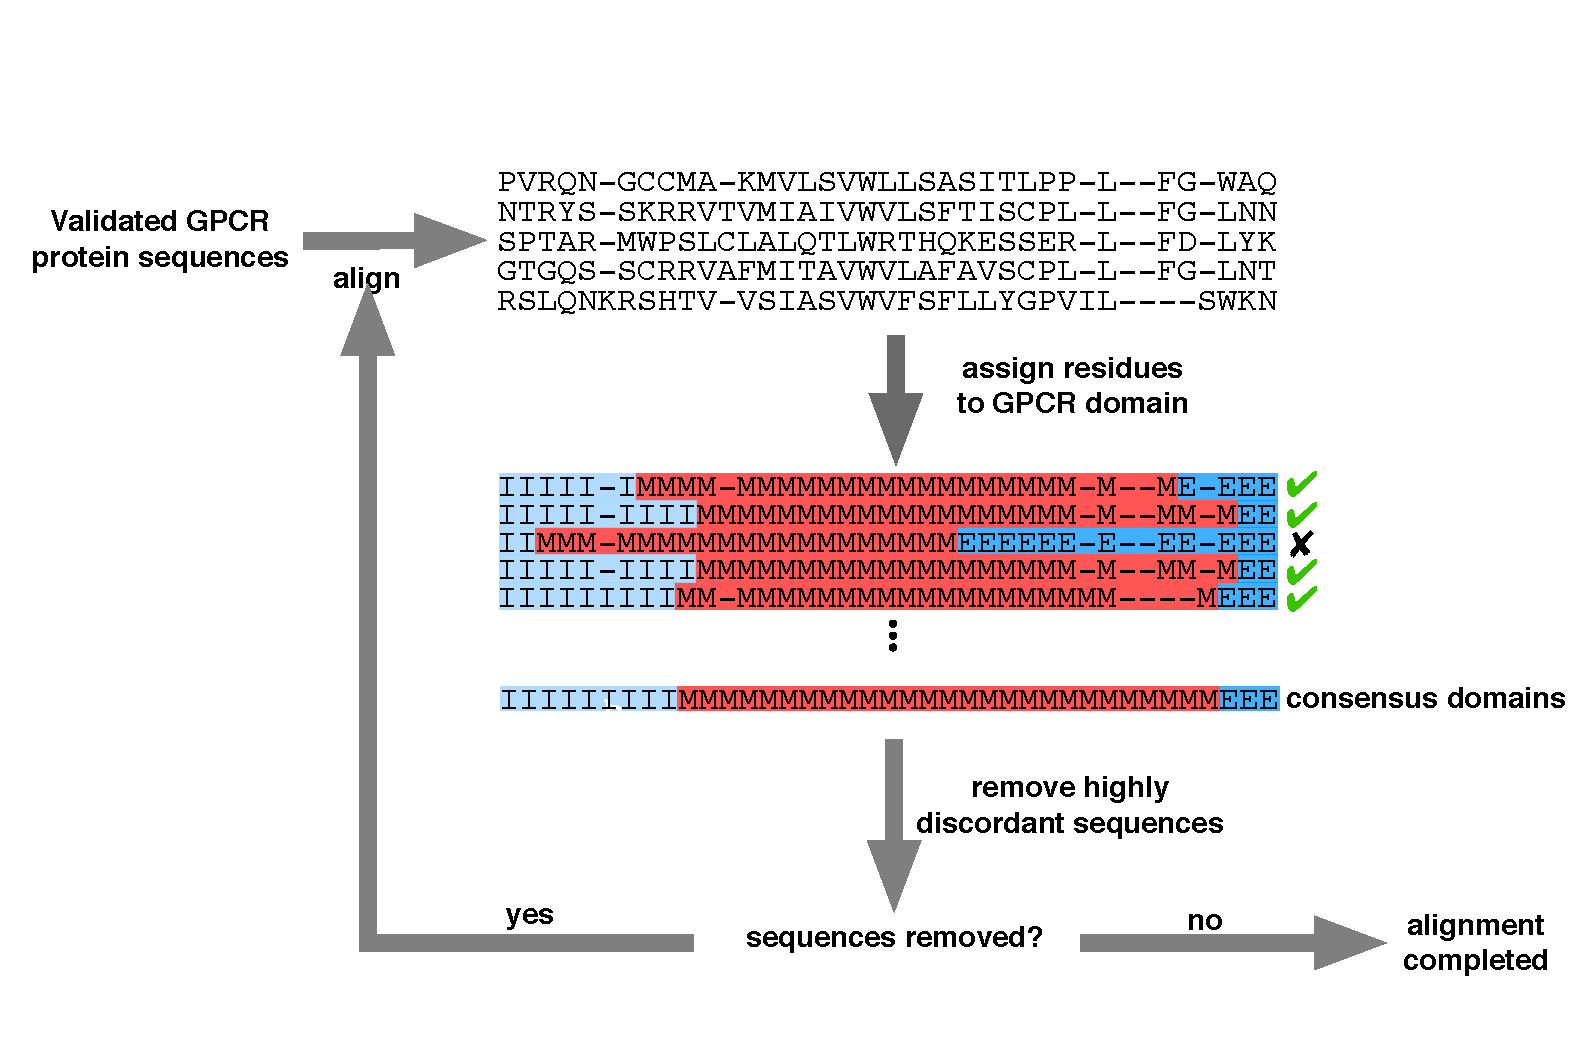
\includegraphics[width=18cm]{figures/alignment_flowchart.pdf}}
	\caption{\label{flowchart} Iterative alignment strategy to create a structurally-curated MSA of vertebrate biogenic amine receptors. A total of 3464 sequences were initially input (``Validated GPCR protein sequences''), and the final MSA contained 3039 protein sequences. Residues marked with ``I'' represent intracellular residues, those marked with ``M'' represent transmembrane residues, and those marked with ``E'' represent extracellular residues. MSA gaps were regarded as missing data when determining each column's consensus structural domain. Sequenced were removed (``remove highly discordant sequences'') if $\geq 5\%$ of columns belonged to a different structural domain than the respective consensus domain.}
\end{figure}


\newpage


\begin{figure}[htbp]
	\centerline{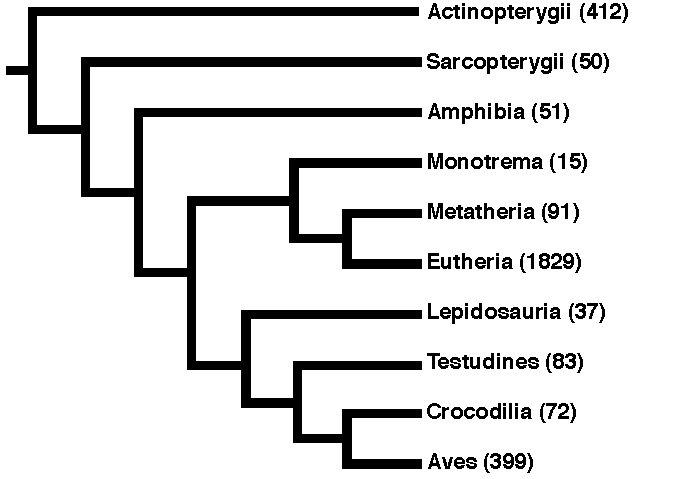
\includegraphics[width=7cm]{figures/taxonomic_distribution.pdf}}
	\caption{\label{taxa_dist} Cladogram of the taxonomic distribution of all sequences in the final structurally-curated MSA. All sequences belonged to the \emph{Euteleostomi} clade of jawed vertebrates. Numbers in parentheses indicate the total number of biogenic amine receptors in the respective clade. We note that our MSA is particularly enriched for sequences from Eutherian (placental mammal) species, likely due to the stringent filters we applied to sequence collection which favored fully-sequenced genomes.}
\end{figure}

\vspace{3cm}

\begin{table}[htbp]
	\centering
	\begin{tabular}{l c l l c}
		\hline\noalign{\smallskip}
		\multicolumn{1}{c}{MSA} & \multicolumn{1}{c}{Partitions?} & \multicolumn{1}{c}{$\ln L$} & \multicolumn{1}{c}{k} & \multicolumn{1}{l}{$\Delta$AIC} \\
		\hline\noalign{\smallskip}
		Structural Masked & Yes & -505500.8 & 6115 & 0 \\
		Structural Masked & No & -515991.7 & 6095 & 1752 \\  
		Structural Unmasked & Yes & -515343.6 & 6115 & 19685 \\
		Structural Unmasked & No & -515991.7 & 6095 & 20941 \\ 
		Naive & No &  -589703.7 & 6945 & 170047 \\
		\noalign{\smallskip}\hline\noalign{\smallskip} 
	\end{tabular}
	\caption{\label{tab:phylo_AIC} $\Delta$AIC scores relative to the best performing for phylogenies. The column labeled ``Partitions?'' indicates whether phylogenetic inference was conducted with distinct TM (transmembrane) and EM (extramembrane) partitions. AIC is computed as AIC $= 2(k - \ln L)$, where $k$ is the number of free parameters of the model, and $\ln L$ is the log-likelihood \citep{Akaike1974,BurnhamAnderson2004}. AIC scores are reported here relative to the phylogeny with the lowest AIC score (structural masked with partitions), representing the best-fitting phylogeny.}
\end{table}


\newpage

\begin{figure}[htbp]
	\centerline{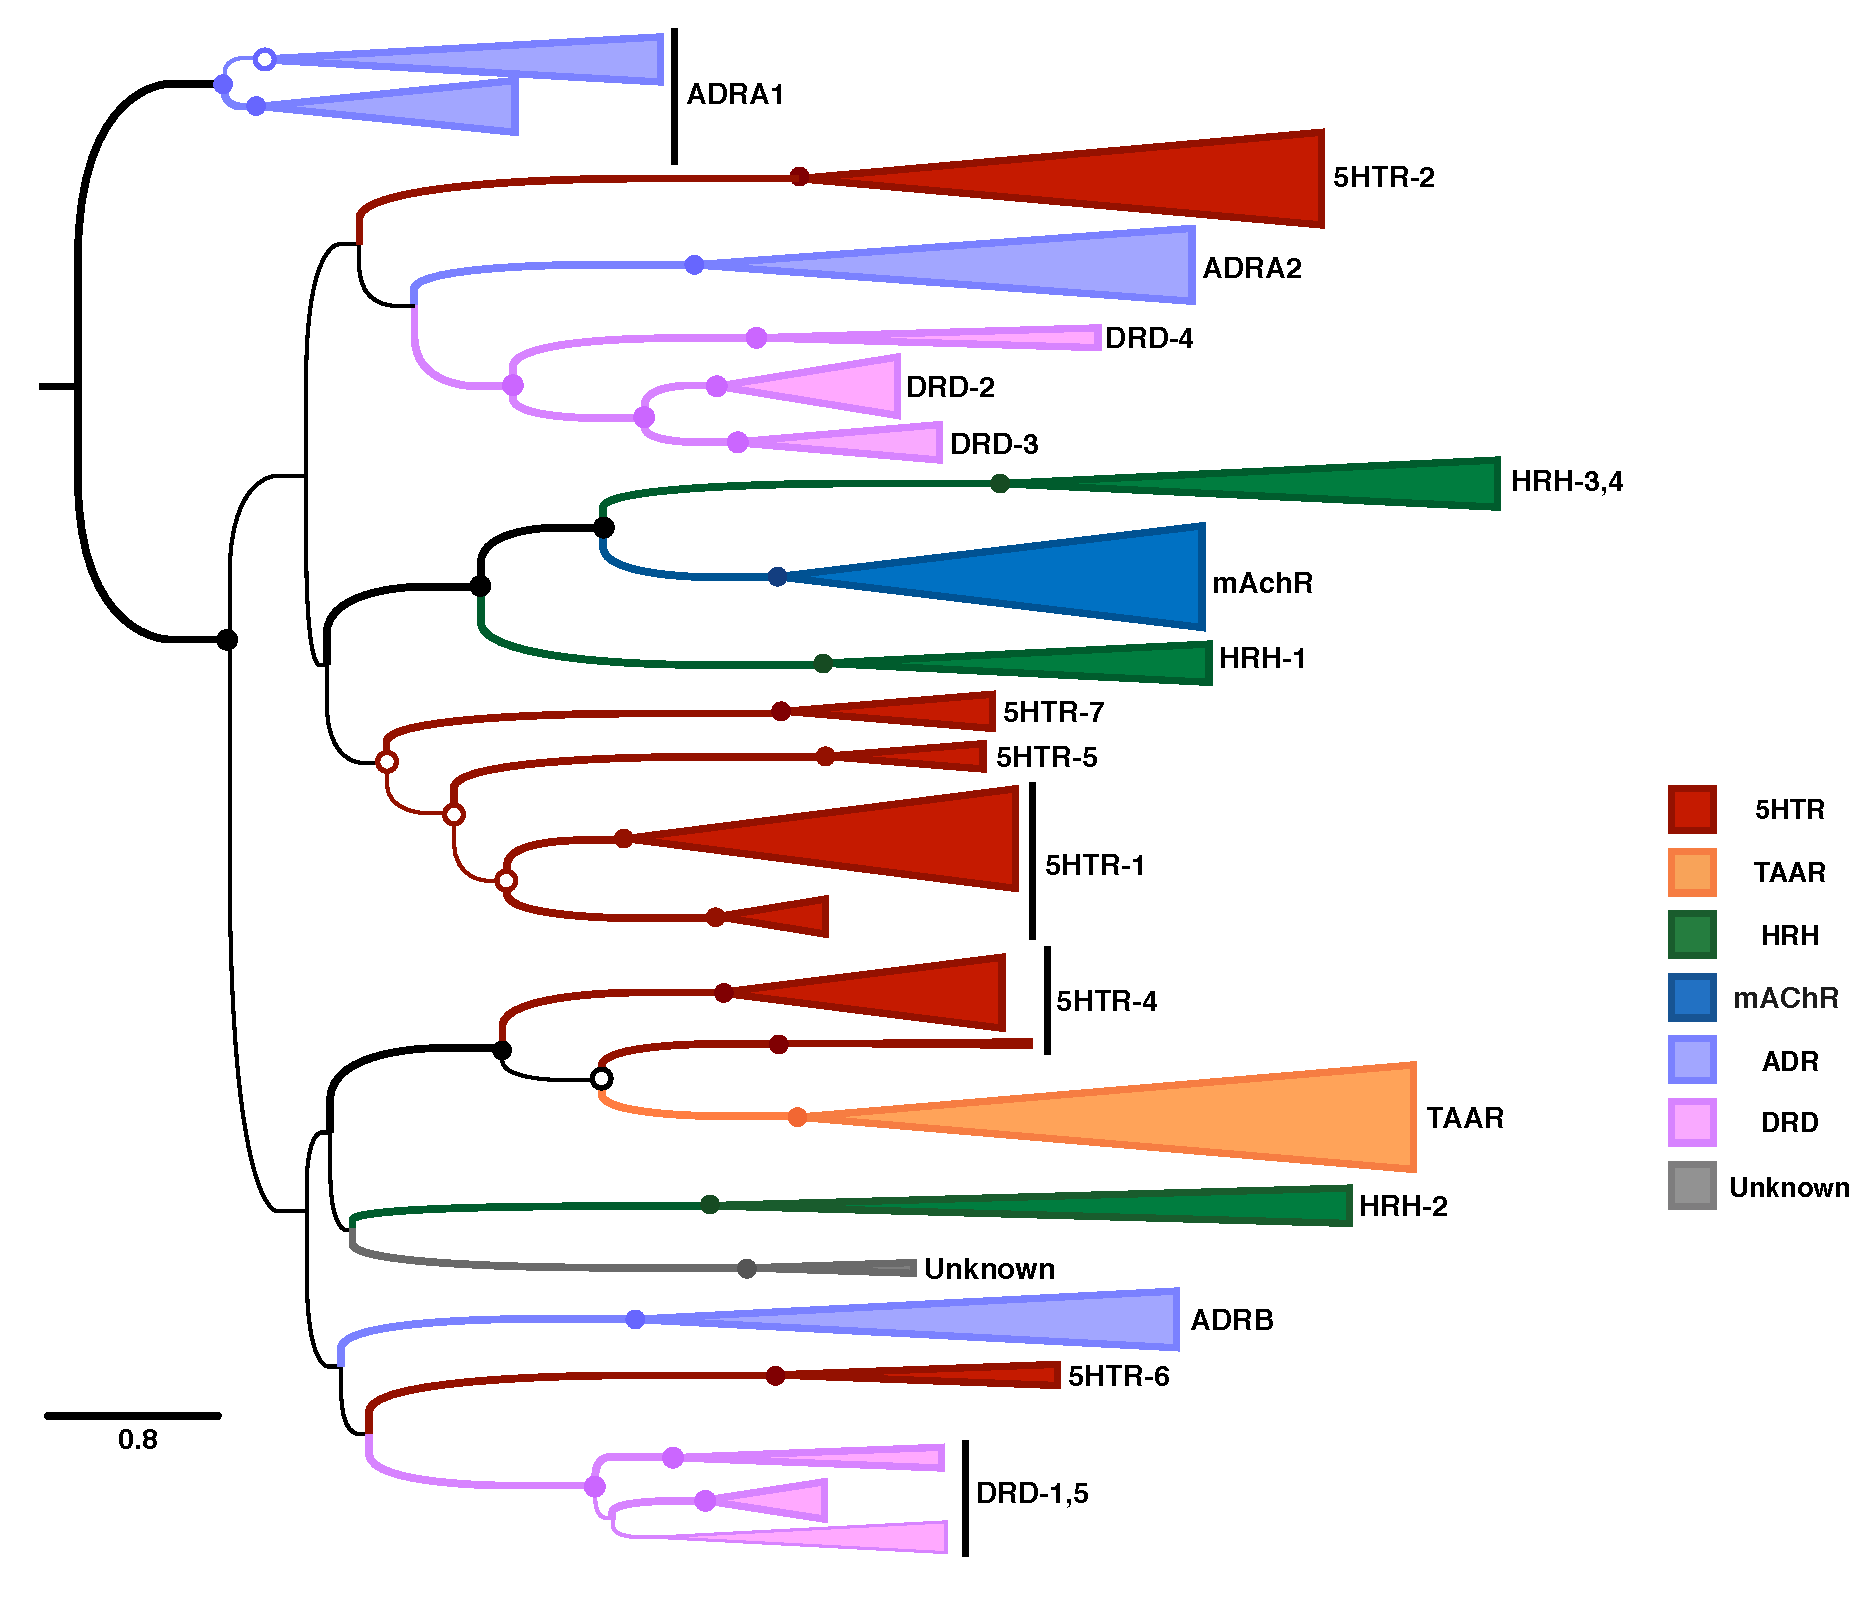
\includegraphics[width=18cm]{figures/masked_part_phylogeny.pdf}}
	\caption{\label{phylogeny} Maximum likelihood phylogeny of vertebrate biogenic amine receptors built using the masked structural MSA in RAxML. Nodes with open circles indicate $\geq 50\%$ bootstrap support, and nodes with closed circles and thick lines indicate $\geq 90\%$ bootstrap support. Bioaminergic receptors are abbreviated as 5HTR, serotonin receptors; TAAR, trace amine-associated receptors; HRH, histamine receptors; mAChr, muscarinic acetylcholine receptors; ADR, adreneric receptors; and DRD, dopamine receptors. The clade labeled ``Unknown'' could not be clearly identified as one of the major receptor types and may represent a novel biogenic amine receptor clade.}
\end{figure}


\newpage

\begin{figure}[htbp]
	\centerline{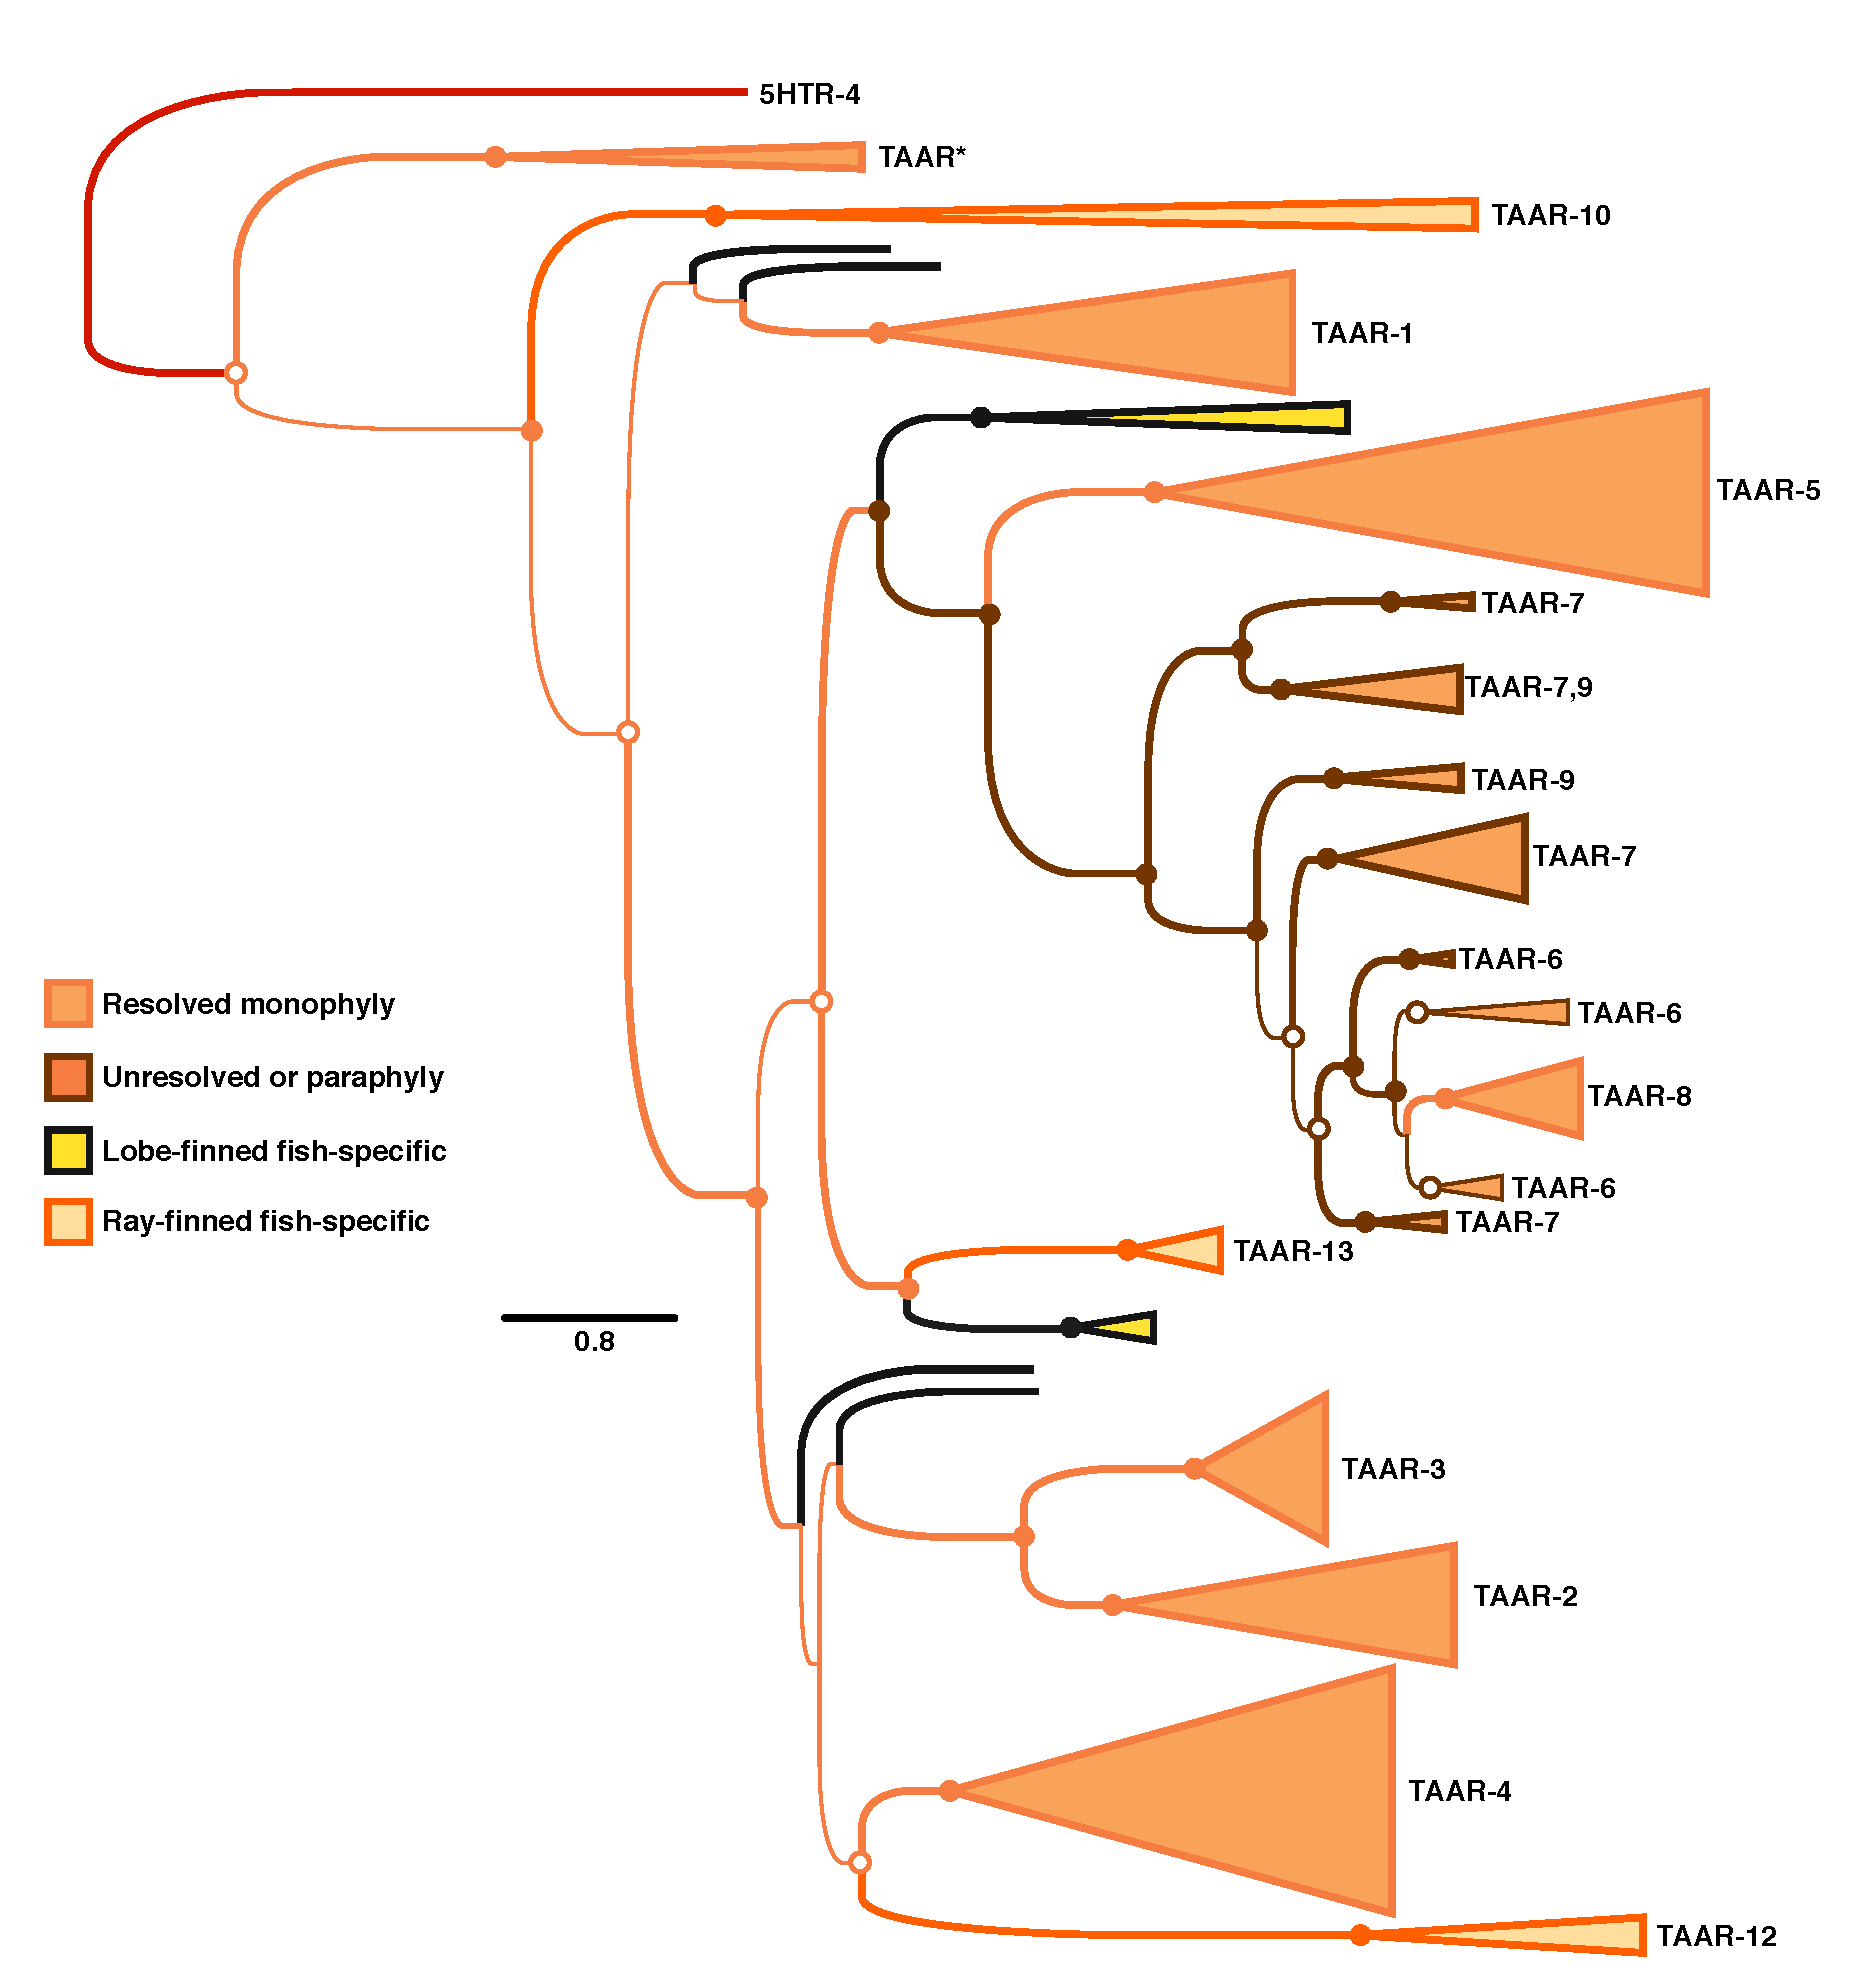
\includegraphics[width=15cm]{figures/taar_phylogeny.pdf}}
	\caption{\label{taar_tree} Subclade of the TAAR receptors within the phylogeny shown in Figure~\ref{phylogeny}. Nodes with open circles indicate $\geq 50\%$ bootstrap support, and nodes with closed circles and thick lines indicate $\geq 90\%$ bootstrap support.}
\end{figure}


% % % % % % % % % % % %    OVERFLOW    % % % % % % % % % % % % % %
 %However, according to this algorithm, sequences in which up to 5\% of positions do not match the consensus domain are retained. Therefore, certain residues which lie at domain boundaries may be improperly aligned with regards to structure. Thus, we created a modified version of this structural alignment in which all residues whose GPCRHMM-assigned domain did not agree with its respective column's consensus domain were masked. 
 %Therefore, while the final alignment might contain a few improperly aligned residues, this issue is avoided in the masked alignment as each column contains strictly properly-aligned residues.  
 %Therefore, we adopted a novel alignment strategy to ensure that the resulting alignment accuractely reflected the highly conserved overarching GPCR structure. We began by assigning, again using GPCRHMM \citep{Wistrand2006}, 
 %as well as solidify existing hypotheses regarding biogenic amine receptor evolution with a highly robust statistical framework.
%Next, using the GPCRHMM-determined residue domains, we determined the consensus structural domain for each alignment column, and we discarded all sequences in which 5\% of columns did not match this consensus structure. We then realigned the remaining sequences, performing this strategy until no sequences were discarded. The final structurally-curated MSA contained 3039 sequences. In addition to this final alignment, we additionally created a ``masked'' alignment, in which protein residues which did not conform to their respective consensus domains were replaced with a ``?'', thus effectively replacing these positions with an ambiguous character. Therefore, while the final alignment might contain a few improperly aligned residues, this issue is avoided in the masked alignment as each column contains strictly properly-aligned residues.  






\end{document}